%%%%%%%%%%%%%%%%%%%%%%%%%%%%%%%%%%%%%%%%%%%%%%%%%%%%%%%%%%%%%%%
%
% Welcome to Overleaf --- just edit your LaTeX on the left,
% and we'll compile it for you on the right. If you open the
% 'Share' menu, you can invite other users to edit at the same
% time. See www.overleaf.com/learn for more info. Enjoy!
%
%%%%%%%%%%%%%%%%%%%%%%%%%%%%%%%%%%%%%%%%%%%%%%%%%%%%%%%%%%%%%%%
\documentclass[12pt,a4paper,oneside]{book}


\usepackage[T1]{fontenc}
\usepackage[utf8]{inputenc}
\usepackage{arabtex}
\usepackage{utf8}
\setcode{utf8}
\usepackage{babel}
\usepackage{svg}
\usepackage{amsmath}
\usepackage{amsthm}
\usepackage{amssymb}
\usepackage{tikz}
\usepackage{tcolorbox}
\usepackage{tabularx}
\usetikzlibrary{calc}
\usepackage[french,ruled,vlined]{algorithm2e}
\usepackage{rotating}
\usepackage{bbding}
\usepackage{cite}
\usepackage{lscape,graphicx}
\usepackage{rotating}
\usepackage{setspace}
\usepackage{sectsty}
\usepackage{dsfont}
\usepackage{ifpdf}
\usepackage{subfigure}
\usepackage{epsfig}
\usepackage{float}
\usepackage{titlesec}
\usepackage{multibib}
\usepackage{fancyhdr}
\usepackage{lipsum}
\usepackage{soul}
\usepackage[paperwidth=210mm,paperheight=297mm,tmargin=15mm,lmargin=20mm]{geometry}
%
\renewcommand{\topfraction}{0.9}
\renewcommand{\textfraction}{0.1}
\renewcommand{\floatpagefraction}{0.8}
%

\usepackage{hyperref}


\urlstyle{same}

\setlength{\headheight}{30pt}
\pagestyle{fancy}% \renewcommand{\chaptermark}[1]{\markboth{#1}{}}
\renewcommand{\chaptermark}[1]{\markboth{\MakeUppercase{#1}}{}}
\renewcommand{\sectionmark}[1]{\markright{\MakeUppercase{\thesection.\ #1}}}


%
% \renewcommand{\sectionmark}[1]{\markright{#1}}
%\renewcommand \thesection{\Roman{section}.}
%\renewcommand \thesubsection{\alph{subsection}.}
%
%\newcommand{\helv}{%
%\fontfamily\fontsize{9}{11}\selectfont}

%

% Clear Header Style on the Last Empty Odd pages
\makeatletter
  \def\cleardoublepage{\clearpage\if@twoside \ifodd\c@page\else%
      \hbox{}%
       \thispagestyle{empty}%              % Empty header styles
       \newpage%
       \if@twocolumn\hbox{}\newpage\fi\fi\fi}
\makeatother


\fancyhead[RE]{\textit{\nouppercase{\leftmark}}}
\fancyhead[LO]{\textit{\nouppercase{\rightmark}}}
\fancyhead[LE,RO]{\thepage}

\renewcommand{\headrulewidth}{0pt}
\renewcommand{\footrulewidth}{0pt}
%
\setcounter{secnumdepth}{4}
\setcounter{tocdepth}{4}
%

%
\def\ds{\displaystyle}
\def\dir{./figures}

%


%\setlength\topmargin{0in}
%\setlength\topmargin{0in}
%

%
% Remove page numbering from first page Bibliography
%
%%%%%%%%%%%%%%%%%%%%%%%%% Page de titre %%%%%%%%%%%%%%%%%%%%%%%
\def\baselinestretch{1.5}


\usepackage{listings}
\usepackage{caption}
\usepackage{longtable}

\usepackage{geometry}
\usepackage{booktabs}

\geometry{
    letterpaper,
    left=1.5cm,
    right=1.5cm,
    top=1.5cm,
    bottom=1.5cm
}

\usepackage{afterpage}

\newcommand\blankpage{%
    \null
    \thispagestyle{empty}%
    \addtocounter{page}{-1}%
    \newpage}


\usepackage[acronym]{glossaries}

\usepackage{lmodern}


\newenvironment{dedication}
  {%\clearpage           % we want a new page          %% I commented this
   \thispagestyle{empty}% no header and footer
   \vspace*{\stretch{1}}% some space at the top
   \itshape             % the text is in italics
   \raggedleft          % flush to the right margin
  }
  {\par % end the paragraph
   \vspace{\stretch{3}} % space at bottom is three times that at the top
   \clearpage           % finish off the page
  }


  



%\makenoidxglossaries 

%\newglossaryentry{latex}
%{
       % name=latex,
        %description={Is a mark up language specially suited for scientific documents}
%}



%\selectlanguage{English}



\hypersetup{
    colorlinks=true,
    linkcolor=black,
    filecolor=magenta,      
    urlcolor=cyan,
    pdfauthor={Name},  %put your name here
    pdftitle={PDF_TTILE},  %PDF title
    pdfpagemode=FullScreen,
    }



\begin{document}



\definecolor{codegreen}{rgb}{0,0.6,0}
    \definecolor{codegray}{rgb}{0.5,0.5,0.5}
    \definecolor{codepurple}{rgb}{0.58,0,0.82}
    \definecolor{backcolour}{rgb}{0.95,0.95,0.92}
    
    \lstdefinestyle{mystyle}{
        backgroundcolor=\color{backcolour},   
        keywordstyle=\color{magenta},
        numberstyle=\tiny\color{codegreen},
        stringstyle=\color{codepurple},
        basicstyle=\ttfamily\footnotesize,
        breakatwhitespace=false,         
        breaklines=true,                 
        captionpos=b,                    
        keepspaces=true,                 
        numbers=left,                    
        numbersep=5pt,                  
        showspaces=false,                
        showstringspaces=false,
        showtabs=false,                  
        tabsize=2
    }




%
\thispagestyle{empty}

\includegraphics[scale=0.08]{Logos/Logo_INPT.png} 
         \hspace{11cm}  

\includegraphics[scale=0.1]{Logos/Logo_ANRT.jpg}
        
\vspace{0.9cm}
\begin{center}
{\large \textsc{\textbf{Mémoire du projet de fin d'études}}}\\[0.1cm]
{\large \textsc{Pour L'obtention du Diplôme d'Ingénieur d'État}}\\[0.1cm]
{\large \textsc{\textit{Filière: XXXXXXXXXXXX}}} \\[0.05cm] 
\vspace{-0.04cm}
% Title
\rule{\linewidth}{0.3mm} \\[0.4cm]   % à ajuster l'éspace en cas de besoin: [1cm]
 { \huge \textbf{ Titre de Projet }} \\[0.15cm] 
\rule{\linewidth}{0.3mm} \\[0.4cm]
\vspace{0.4cm}


\includegraphics[scale=0.075]{Logos/Company_Logo_Expl.png}  %change the scale to suit your logo

\vspace{1cm}

% Author and supervisor
\noindent
\begin{minipage}{0.9\textwidth}
    \vspace{-7mm}
  \begin{flushleft} \large
    \emph{Réalisé par :}\\
    Mme / M. Xxxx \textsc{XXXX} %\& Mme / M. Xxxx \textsc{XXXX}  %Au cas de binôme, remove the % \\
  \end{flushleft}
\end{minipage}
\begin{minipage}{0.4\textwidth}

\end{minipage}\\[0.6cm]

{\large \textit{Soutenu le XX Juillet 20XX, devant le jury composé de : }}\\[0.5cm]


\begin{tabular}{p{1cm}lll}
 & \large M / Mme. Xxxx \textsc{XXXX}  & \large INPT & \large - Examinateur/trice \\[0.1cm]
 & \large M / Mme. Xxxx \textsc{XXXX}  & \large INPT & \large - Examinateur/trice \\[0.1cm]
 & \large M / Mme. Xxxx \textsc{XXXX}  & \large INPT & \large - Encadrant/e \\[0.1cm]
  & \large M / Mme. Xxxx \textsc{XXXX}  & \large Entreprise & \large - Encadrant/e \\[0.1cm]
 
\end{tabular}

\vspace{0.5cm}

\includegraphics[scale=0.6]{Logos/ZLAFA.png}


\textsc{Agence National de Réglementation des Télécommunications}\\
\textsc{Institut National des Postes et Télécommunications}
% Bottom of the page

%\vspace{0.3cm}
{\large Promotion : 20XX/20XX}
   
\end{center}


 %FRENCH ONE


\thispagestyle{empty}

\includegraphics[scale=0.08]{Logos/Logo_INPT.png} 
         \hspace{11cm}  

\includegraphics[scale=0.1]{Logos/Logo_ANRT.jpg}
        
\vspace{0.9cm}
\begin{center}
{\large \textsc{\textbf{Thesis of the end-of-study project}}}\\[0.1cm]
{\large \textsc{To obtain the State Engineering Diploma}}\\[0.1cm]
{\large \textsc{\textit{Major: Innovation \& AMOA}}} \\[0.05cm] 
\vspace{-0.04cm}
% Title
\rule{\linewidth}{0.3mm} \\[0.4cm]   % à ajuster l'éspace en cas de besoin: [1cm]
 { \huge \textbf{ Green IT Integration in DevOps }} \\[0.15cm] 
\rule{\linewidth}{0.3mm} \\[0.4cm]
\vspace{0.4cm}


\includegraphics[scale=0.28]{Logos/ob.png}  %change the scale to suit your logo

\vspace{1cm}

% Author and supervisor
\noindent
\begin{minipage}{0.9\textwidth}
    \vspace{-7mm}
  \begin{flushleft} \large
    \emph{Authored by :}\\
    Mr. Imad \textsc{EL BOUHATI} %\& Mr/Mrs/Ms. Xxxx \textsc{XXXX}  %Au cas de binôme, remove the % \\
  \end{flushleft}
\end{minipage}
\begin{minipage}{0.4\textwidth}

\end{minipage}\\[0.6cm]

{\large \textit{Defended on July XX, 2024, before the jury composed of :}}\\[0.5cm]


\begin{tabular}{p{1cm}lll}
 & \large Mr. / Mrs. Xxxx \textsc{XXXX}  & \large INPT & \large - Examiner \\[0.1cm]
 & \large Mr. / Mrs. Xxxx \textsc{XXXX}  & \large INPT & \large - Examiner \\[0.1cm]
 & \large Mrs. Charifa \textsc{HANIN}  & \large INPT & \large - Supervisor \\[0.1cm]
  & \large Mr. Amine \textsc{AJA}  & \large Orange Business & \large - Supervisor \\[0.1cm]
 
\end{tabular}

\vspace{0.5cm}

\includegraphics[scale=0.55]{Logos/ZLAFA.png}


\textsc{Agence National de Réglementation des Télécommunications}\\
\textsc{Institut National des Postes et Télécommunications}
% Bottom of the page

%\vspace{0.3cm}
{\large Class of : 2023/2024}
   
\end{center}


 % ENGLISH

\afterpage{\blankpage}  %page vide obligatoire

\frontmatter


\chapter*{Dedicated to}
\addcontentsline{toc}{chapter}{Dedication}

\begin{dedication}
  
  \hspace{1em} I humbly dedicate this work to my dear mother, who gave me life, love, courage, and a reason to live.
  I also wish to express my gratitude to my father for his support and sacrifices.
  \vspace{\baselineskip}
  \par   %% or a blank line
  
  A big thank you to my two dear sisters, Alae and Samia, whom I love so much,
  to all my friends with whom I have shared moments of joy and happiness, as well as to my entire extended family and to all those who love me.

  \vspace{\baselineskip}
  \hspace*{\fill} \usefont{T1}{LobsterTwo-LF}{bx}{it} Imad
  
\end{dedication}


\chapter*{Acknowledgments}
\addcontentsline{toc}{chapter}{Acknowledgments}


First and foremost, I would like to express my gratitude to Allah the Almighty for giving me the strength and patience necessary to complete this project.

I would like to extend my sincerest thanks to my supervisor, Mrs. Charifa HANIN, for her competent assistance, patience, and encouragement. Her critical feedback has been invaluable in structuring my work and improving the quality of its various sections.

I also want to express my appreciation to my mentor, Mr. AJA Amine, for his immense support, the quality of his guidance, and for all the advice and information he provided with unmatched professionalism and patience.

A big thank you is also owed to Mr. MOUSTACHI Mouhsine, for offering me the opportunity to join his team and for his support.

I would also like to thank Mr. EDDAHBY Mohamed Amine, Mr. ECHARJI Abderrahman, Mr. OUCHEN Othman, Mr. EL ALJ Mohamed Taieb, Mr. EL IDRISSI Hicham, Ms. EL IBRAHIMI Dounia, Mr. OUADHDHAFE Marouane, and all the engineers in the DevOps team for their invaluable assistance, encouragement, and for making my internship at Orange Business a very enriching experience.

I wish to express my sincere gratitude to the members of the jury for the honor they bestow upon me by taking the time to read and evaluate my work.

I would also like to thank the pedagogical and administrative team at INPT for their dedication and contribution to our excellent education.

Finally, I would like to thank all the individuals who have contributed, directly or indirectly, to the completion of this work.


\chapter*{Résumé}
\addcontentsline{toc}{chapter}{Résumé}


Ce rapport reflète le travail réalisé chez Orange Business Maroc dans le cadre de mon projet de fin d'études pour le diplôme d'ingénieur en Télécommunications et Technologies de l'Information.

Dans un contexte où les architectures distribuées et les pratiques de développement agile dominent la conception des applications, intégrer les principes de Green IT dans les pratiques DevOps est devenu essentiel. Cette évolution témoigne de l'importance croissante accordée à la durabilité environnementale dans le secteur de la technologie.

En se concentrant sur la surveillance de la consommation d'énergie et des émissions de CO$_2$ de l'infrastructure, nous mettons en lumière une préoccupation croissante pour l'empreinte écologique de nos systèmes informatiques. Cette prise de conscience a conduit à l'adoption de mesures proactives telles que l'utilisation de Kepler, Prometheus et Grafana pour surveiller et visualiser ces métriques environnementales.

Mon projet de fin d'étude vise à mettre en place Kepler pour surveiller la consommation énergétique et les émissions de CO$_2$ de Kubernetes, et à l'intégrer dans la chaîne CI/CD.

\noindent\rule[2pt]{\textwidth}{0.5pt}

{\textbf{Mots-clés :}}
Green IT, DevOps, Kepler, Prometheus, Grafana, Kubernetes, CI/CD.

\noindent\rule[2pt]{\textwidth}{0.5pt}

% \cleardoublepage
%

\chapter*{Summary}
\addcontentsline{toc}{chapter}{Summary}

This report reflects the work carried out at Orange Business Morocco as part of my final project for the engineering degree in Telecommunications and Information Technologies.

In a context where distributed architectures and agile development practices dominate application design, integrating Green IT principles into DevOps practices has become essential. This evolution underscores the increasing importance placed on environmental sustainability in the technology sector.

By focusing on monitoring energy consumption and CO2 emissions of the infrastructure, we highlight a growing concern for the ecological footprint of our computer systems. This awareness has led to the adoption of proactive measures such as using Kepler, Prometheus, and Grafana to monitor and visualize these environmental metrics.

My final project aims to implement Kepler to monitor energy consumption and CO2 emissions of Kubernetes, and integrate it into the CI/CD pipeline.

\noindent\rule[2pt]{\textwidth}{0.5pt}

{\textbf{Keywords:}}
Green IT, DevOps, Kepler, Prometheus, Grafana, Kubernetes, CI/CD. 

\noindent\rule[2pt]{\textwidth}{0.5pt}

% \cleardoublepage
%

\chapter*{\RL{ملخص}}
\addcontentsline{toc}{chapter}{Arabic Abstract}

\begin{RLtext}
يعكس هذا التقرير العمل الذي قمت به في أورانج بيزنس المغرب في إطار من مشروعي الختامي للحصول على شهادة مهندس دولة في الاتصالات وتكنولوجيا المعلومات.

 في سياق تهيمن فيه الهياكل الموزعة وممارسات التطوير السريعة على تصميم التطبيقات، أصبح دمج مبادئ تكنولوجيا الخضراء في ممارسات \LR{DevOps} أمراً ضرورياً. يؤكد هذا التطور على الأهمية المتزايدة التي تحظى بها الاستدامة البيئية في قطاع التكنولوجيا.
  
 وقد أدى هذا الوعي إلى اعتماد تدابير استباقية مثل استخدام \LR{Kepler} و \LR{Prometheus} و \LR{Grafana} لمراقبة هذه المقاييس البيئية وتصورها.
 
 يهدف مشروعي الختامي إلى تطبيق \LR{Kepler} لمراقبة استهلاك الطاقة وانبعاثات ثاني أكسيد الكربون في \LR{Kubernetes} و دمجه في سلسلة \LR{CI/CD}.
\end{RLtext}

\noindent\rule[2pt]{\textwidth}{0.5pt}

\begin{RLtext} 

{\textbf{الكلمات المفتاحية:}} \LR{Green IT, DevOps, Kepler, Prometheus, Grafana, Kubernetes, CI/CD}
\\

\end{RLtext}

\noindent\rule[2pt]{\textwidth}{0.5pt}


% \cleardoublepage
%






\listoffigures
\addcontentsline{toc}{chapter}{List of Figures} 
%figures are added automatically here

\listoftables
\addcontentsline{toc}{chapter}{List of Tables} 
%tables are added automatically here

%\lstlistoflistings
%\addcontentsline{toc}{chapter}{List of Listings} 
%Code snippets are added automatically here

\tableofcontents
\addcontentsline{toc}{chapter}{Table of Contents}
%contents are added automatically here

\mainmatter

%debut of chapters
\chapter*{General Introduction}
\addcontentsline{toc}{chapter}{General Introduction}

Modern applications are typically designed with distributed architectures and developed using agile methodologies. These continuous integration and delivery (CI/CD) practices play a crucial role in efficiently managing the software lifecycle in terms of speed and effectiveness. However, despite this efficiency, security is often overlooked in the CI/CD workflow, particularly regarding concerns related to environmental footprint.

After deploying an application in a real production environment, additional security measures are needed to ensure its protection. The use of Green IT practices, such as integrating metrics for energy consumption and CO$_2$ emissions into the CI/CD pipeline, is becoming increasingly important to ensure the environmental sustainability of technological infrastructures.

My thesis project fits into this context, aiming to automate the monitoring of energy consumption and CO$_2$ emissions in DevOps infrastructures using Kepler. 

\vspace{10pt} % Add space between paragraphs

This report synthesizes the work done throughout my internship period, structured into four chapters covering various aspects of the project. 

\vspace{10pt} 

The first chapter introduces the project context, objectives, and the approach and planning followed. 

\vspace{10pt} 

The second chapter focuses on the project's requirements analysis, while the third chapter addresses the technological choices. 

\vspace{10pt} 

Finally, the fourth chapter presents the project's final structure in detail, along with an overview of the achievements. The report concludes with a summary and a list of bibliographical references.


\chapter{General Project Context}
\label{chap:General Project Context}

% "*" makes the section unnumbered

\section{Introduction}

This chapter aims to conduct an initial exploration of the project, in order to better understand the system requirements, and to position the project within its organizational and contextual environment. It provides an overview of the hosting organization Orange Business Morocco, then reveals the general theme of the project by introducing its intentions and specifications, followed by the various approaches applied, including the recommended methodology for project management and the resulting planning.


\newpage


\section{Presentation of host organization}



\subsection{Company Overview}

\begin{figure}[H] 
    \centering
    
\includegraphics[width=7cm]{Logos/ob.png}
    \caption{OBS logo}
    %\label{fig:my_label} %Optional (If you want to reference the figure in later chapters)
\end{figure}

In 2000, following the opening of the telecommunications market to competition in Europe, France Télécom, the historic French operator, acquired the British brand Orange. At the same time, the Senegalese group Sonatel was created in the late 1980s, resulting from the merger of the Office des Postes et Télécommunications and TéléSenegal. Sonatel was privatized in 1997 and integrated into France Télécom's capital.

In France, France Télécom, quickly becoming a leader thanks to the quality of its networks, gradually unified all the group's subsidiaries under the name Orange. By 2009, Orange had a presence in more than 30 countries and served over 123 million customers.

On July 1, 2013, following a vote at a general meeting, France Télécom officially changed its name to Orange. This transformation marked a new chapter for the company while retaining a cultural heritage inherited from the public service. France Télécom's historic installations played an important role in the French telephone network, paving the way for the rise of mobile telephony and the beginning of a new revolution: the Internet.

Orange operates in several regions, notably in Europe, Africa, and the Caribbean. In 2019, it was considered the leader or second operator in 75% of the European countries where it is present, and in 83% of the countries in Africa and the Middle East. Orange offers telecommunications equipment and services for individuals, professionals, and businesses.

Orange Business operates in 166 countries and serves its customers in 220 countries and territories (Table 1.1).
\begin{longtable}[c]{| m{4.4cm} | m{11cm} |}
          \hline
          Date of Establishment & 2006 \\
          \hline
          Legal Form & Legal Form \\
          \hline
          Management & Christel Heydemann (CEO, Orange S.A)
          Helmut Reisinger (CEO, Orange Business Services) \\
          \hline
          Headquarters & Paris, France \\
          \hline
          Parent Company & Orange \\
          \hline
          Activity & Telecommunications
          Information Technology Services \\
          \hline
          Subsidiaries & Orange Application for Business, Business et Decision \\
          \hline
          Website & \url{http://www.orange-business.com} \\
          \hline
          \caption{Orange Business Information}\\
\end{longtable}

\subsection{Orange Business Morocco}
Orange Business Morocco is a newly established entity in 2018 in Rabat, specializing in the design and development of application services and system integration in various domains. It works on behalf of various expertise of Orange Business Services. Several companies have provided application services for Orange Business Services, such as Almerys, a health third-party payer operator. OBS IT Morocco is founded to take control of its applications, optimize and rationalize costs, bring development teams closer to business directions, and improve IT solution delivery times for TTM. By following an Agile way of working to deliver functionalities regularly that create the most value and adopting a simple and automated development and production environment to focus on the essentials. OBS IT Morocco uses the cloud, DevSecOps tools, and automated testing and feedback utilization to enrich applications while ensuring a user-centered approach. By guaranteeing versatile, autonomous, and committed teams to manage all activities on their applications (collecting requirements, drafting user stories, development, testing, integration, deployment, support).

\subsection{Organization and Organizational Chart}
OBS Morocco, overseen by a director Mrs. Rym Sahnoun who is the highest authority, is organized into operational poles whose goal is to focus its energies on a daily basis towards customer satisfaction. Teams are organized by Orange business services. I completed my internship in the OBS IT entity managed by Mr. Aarab Abderrahim and specifically Customer Marketing Innovation (Fig. 1.6) in the DevSecOps/TAAS team attached to Mr. Moustachi Mouhcine, IT RUN Manager (see Fig. 1.7).

\begin{figure}[H]
  \centering
  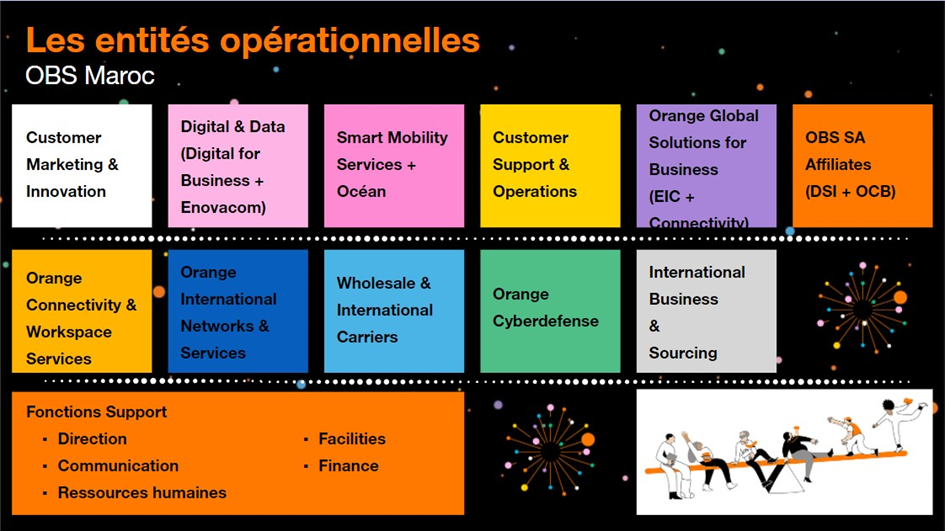
\includegraphics[width=17.5cm]{Figures/entite.png}
  \caption{OBS IT Morocco's operating entities}
  \label{fig:vue-snoc-pos}
\end{figure}

\textbf{CMI}: This is the IT Department of the Orange Group. Its goal is to create efficient software development, entity-oriented, based on the best practices of a software factory (digital factory model). This entity adopts an agile delivery model, possesses a simple and automated development and production environment. It is a versatile, autonomous, and committed team to manage all activities related to the applications entrusted to it: from collecting customer needs and requirements, to writing user stories, through development, testing, and integration, before reaching deployment and support.

\begin{itemize}
  \item Enrich the relationship between companies and their customers through a digital approach and a 360° customer journey.
  \item Exploit machines and communicating objects that transmit real-time data to create new sources of revenue and differentiation.
  \item Make use of the data produced by companies and their customers to innovate and personalize their products and services.
  \end{itemize}
  
\textbf{OCWS}: This entity is composed of 3 poles with different missions. The first center, internationally / in Morocco, manages the operational part. A pre-sales team provides technical assistance to commercial engineers to help them negotiate contracts. A BUILD team's missions include deploying network solutions for customers and offering them the best possible connectivity experience through various technologies such as SDWAN, WIFI, LAN, etc.

\vspace{10pt} 

\textbf{OCD}: This is the entity that designs cybersecurity services that support customers in the Maghreb and West Africa, throughout the life cycle of threats that can impact client companies. They have 5 main missions:
  
  \begin{itemize}
  \item Anticipate the latest threats.
  \item Identify the assets and critical data of customers, prepare the security strategy, and ensure its proper functioning.
  \item Deploy appropriate technology to defend the organization and manage it continuously.
  \item Monitor, qualify, and analyze security alerts to confirm if there has been an incident.
  \item Qualify, contain, and remedy attacks. Thanks to their sectoral expertise, they can offer tailor-made services to meet customer challenges.
  \end{itemize}
  
  \textbf{Orange Connectivity}: Entity responsible for marketing OBS Connectivity data offers (Internet, Ethernet, VPN).
  
  \vspace{10pt} 

  \textbf{Missions in Morocco}: Management of pricing for offers marketed in France and internationally (definition and update of standard prices, calculation of custom prices).
  
  \vspace{10pt} 

  \textbf{OINIS}: Orange International Networks Infrastructures \& Services' mission is to design, deploy, and operate reliable, secure, and high-quality international network infrastructures and services for businesses, wholesale customers (operators), and subsidiaries.

  \vspace{10pt} 

  \textbf{WIN IC}: This is the commercial arm of OINIS. This entity provides international connectivity services to operators and internet service providers worldwide.

  \vspace{10pt} 
  
  \textbf{The Business Unit EIC} (Enriched Interactions and Collaboration): Straddling digital \& data and connectivity, its goal is to design and bring to market communication and collaboration offerings from Orange Business Services: voice solutions, conference solutions, unified communications suites, and contact center solutions.

\section{Project presentation}
\subsection{General project context}
In today's world, ensuring the sustainability of IT practices is paramount. When it comes to IT professionals, it is imperative to prioritize eco-friendly strategies from the outset of the development process.

As a developer, you may not be required to master the intricacies of environmental impact assessments, as there are several reliable tools available to assess the carbon footprint of IT solutions. By integrating these assessments into the CI/CD pipeline and implementing effective remediation strategies, organizations can significantly reduce the environmental cost associated with IT operations.

This includes not only the direct costs of energy consumption but also the broader environmental impact of resource depletion and pollution. Consequently, IT teams have embraced a new approach known as Green IT, which promotes the integration of sustainability principles into IT practices and encourages close collaboration between environmental experts, developers, and IT engineers.

This approach ensures that environmental considerations are addressed at every stage of the development and delivery process, thereby fostering a more sustainable IT ecosystem.

The project is set within this broader context of optimizing Green IT practices at Orange Business Services Morocco. To support this initiative, the DevSecOps team has been recently created within the IT RUN entity to fulfill two main missions:

\begin{itemize}
    \item \textbf{Cloud DevSecOps}: Design, build, and implement Cloud services and DevSecOps tools.
    \item \textbf{REaCT}: Implement the DevOps mindset within the company and support development projects.
\end{itemize}

\begin{figure}[H]
  \centering
  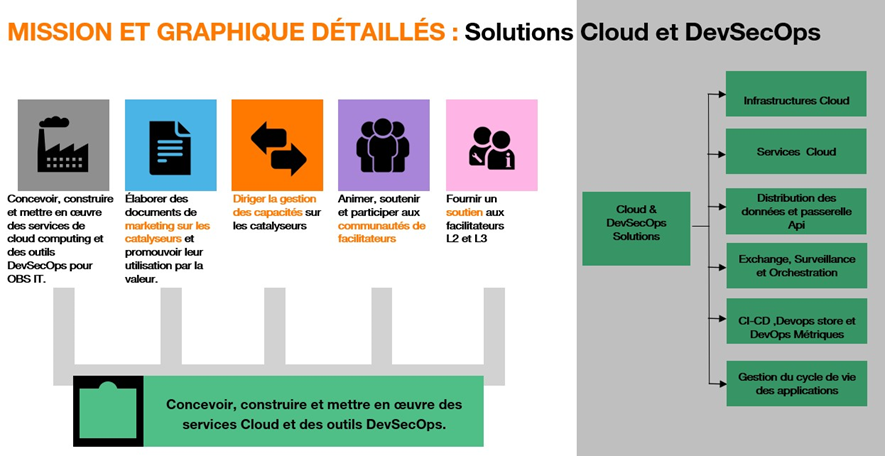
\includegraphics[width=17.5cm]{Figures/mission.png}
  \caption{Cloud \& DevSecOps missions}
\end{figure}
\subsection{Problematic}

While Orange Business Services Morocco has established efficient CI/CD pipelines using GitLab, there is a lack of focus on environmental sustainability and energy efficiency within their DevOps processes. The current approach prioritizes swift software delivery but overlooks the environmental impact of development and deployment activities. This neglect of Green IT principles hinders efforts to reduce energy consumption and carbon emissions associated with the organization's IT infrastructure, particularly its Kubernetes clusters. The challenge lies in integrating Green IT considerations seamlessly into existing DevOps workflows without compromising efficiency or productivity. Thus, the problematic revolves around balancing the need for rapid software delivery with environmental responsibility, requiring the development of strategies and tools to monitor and optimize energy usage and carbon footprint throughout the CI/CD pipeline
\section{Project planning and management}
\subsection{Adopted methodology}

To ensure optimal progress of our project, we have chosen to use the agile Scrum method (illustrated in Fig. 1.10).

\begin{figure}[H]
  \centering
  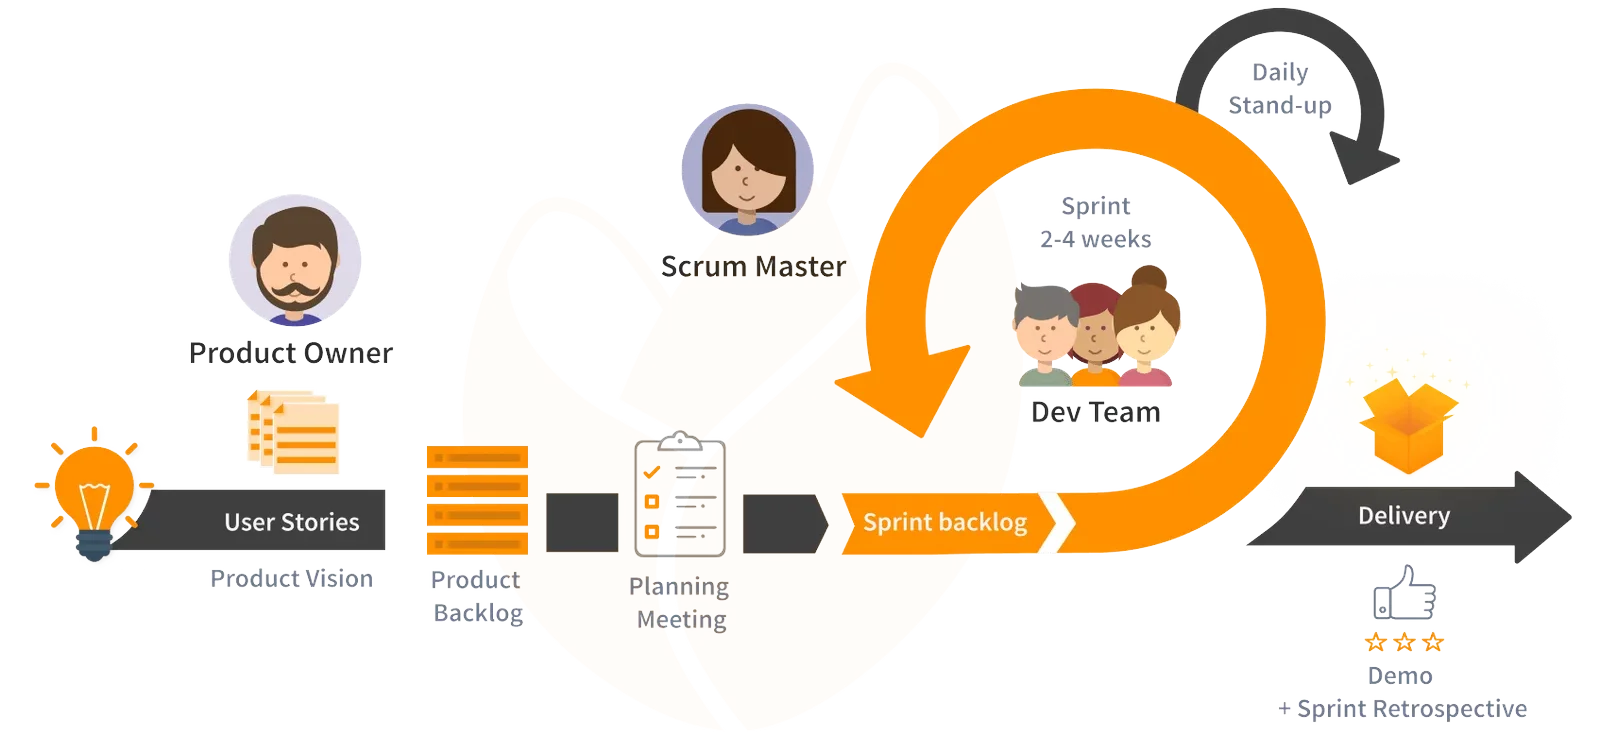
\includegraphics[width=17.5cm]{Figures/scrum.png}
  \caption{Scrum methodology}
\end{figure}

This approach will enable us to best meet the needs of the company while minimizing the risk of delays and ensuring the satisfaction of all stakeholders.

Scrum is an agile project management method that was first introduced in an article by Hirotaka Takeuchi and Ikujiro Nonaka in 1986, published in the Harvard Business Review under the title "The New Product Development Game". It was developed in the 1990s and formalized by Ken Schwaber and Jeff Sutherland in 1995.

The fundamental principle of this method is to iteratively focus on the features to be implemented. The project is divided into functional modules that are developed, tested, and delivered in iterative sequences called "sprints". Each sprint aims to achieve a specific goal, from which the features to be implemented are chosen.

We have adapted the Scrum method to our project by dividing it into sprints of two to three weeks. At the end of each sprint, a meeting is organized with the Scrum Master and the Product Owner to review the work done during the period and set the tasks and objectives for the next sprint. If differences are noted during the inspection, we adapt the process in question. To do this, we have set up weekly meetings led by the Scrum Master, during which each team member presents the status of their tasks, reports any encountered blockers, and outlines the actions to be taken for the next period as well as future prospects. This approach has allowed us to clearly define the objectives for each increment and adapt them as needed, while also allowing us to complete or modify the list of features to be implemented for the upcoming sprints.

\subsection{Project Planning}
Planning is an essential step in project management, as it allows defining the tasks to be performed, setting objectives, coordinating actions, mastering resources, reducing risks, monitoring ongoing actions, and reporting on the project's progress. In our case, we began by breaking down the project into tasks, then proceeded with a risk assessment before establishing a Gantt chart to have an overview of the project's progress.

\subsection{Project Breakdown into Sprints}

The project is divided into sprints, with each sprint being a crucial step in the project's completion.

\begin{figure}[H]
    \centering
    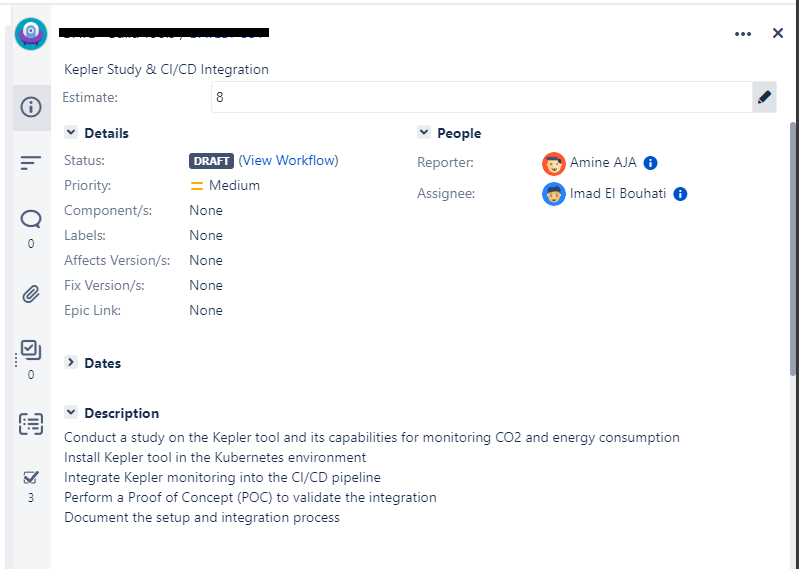
\includegraphics[width=16cm]{Figures/us-1.png}
    \caption{Tasks performed}
\end{figure}

\begin{figure}[H]
  \centering
  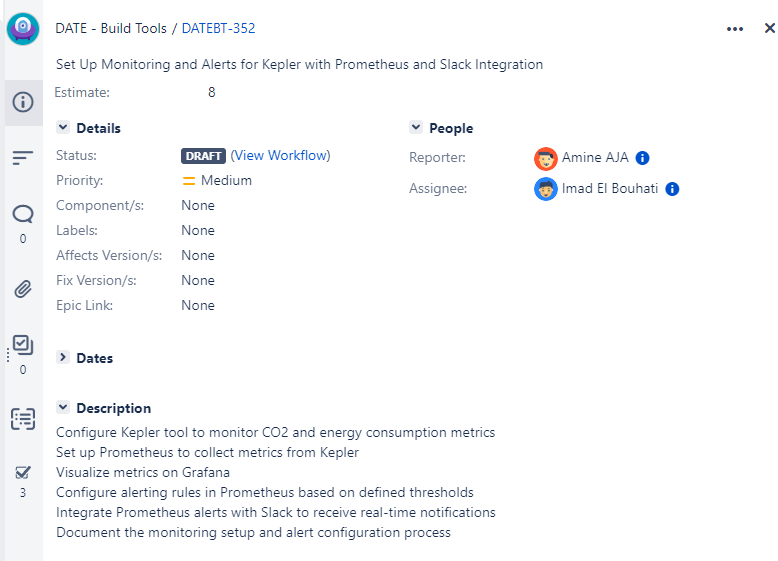
\includegraphics[width=16cm]{Figures/us-2.png}
  \caption{Tasks performed}
\end{figure}

\subsection{Communication Tools}

In the dynamic environment of modern project management, effective communication is paramount to ensure seamless collaboration and timely decision-making. Utilizing robust communication tools can streamline interactions within teams and enhance overall productivity.

\begin{figure}[H]
  \centering
  
\includegraphics[width=3cm]{Logos/microsoft_teams_logo.png}
  \caption{Microsoft Teams Logo}
\end{figure}

Microsoft Teams serves as a cornerstone for communication within our DevSecOps team. This platform offers a comprehensive suite of features, including instant messaging, video conferencing, file sharing, and integration with various productivity tools. Team members can collaborate in real-time, hold meetings, and access project-related resources, fostering efficient communication and collaboration.

\subsection{Internship Progress}

The Gantt chart is a visual presentation method that allows positioning in time the different stages, activities, tasks, and resources involved in a project. Tasks are listed on the rows, while the columns represent days, weeks, or months. The bars symbolizing each task have a length proportional to the expected duration.
\begin{figure}[H]
    \centering
    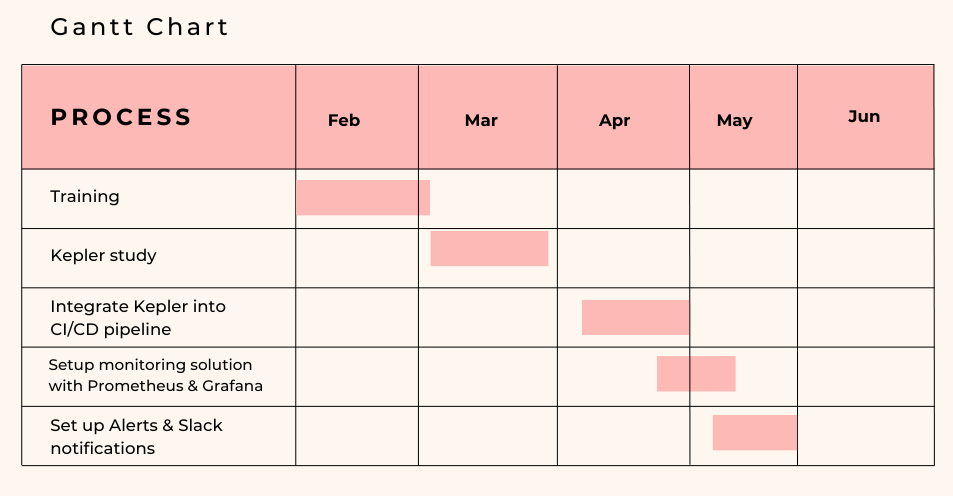
\includegraphics[width=16cm]{Figures/gantt-chart.png}
    \caption{Gantt Chart}
\end{figure}
\section{Conclusion}
In this chapter, we first introduced Orange Business Morocco, the organization involved in the project. Then, we established the general framework of the project before presenting the specific problem to be addressed. We also explained the working method we adopted and provided an overview of the schedule that was followed throughout the project. In the next chapter, we will move on to the functional and non-functional analysis of our project, as well as detailed design. This phase will define the specifications necessary for the development of the overall project architecture.

\chapter{Chapter 2 title}
\label{chap:Chapter 2 title}
\section*{Introduction}


Lorem ipsum dolor sit amet, consectetur adipiscing elit. Praesent nec dapibus justo. Donec sagittis vulputate ante sed porttitor. Suspendisse sit amet nisl massa. Curabitur nec nisl condimentum, egestas ex vitae, dapibus enim. Etiam iaculis, erat faucibus pellentesque sagittis, nisi justo sollicitudin nibh, et condimentum augue massa non turpis. Proin commodo enim fermentum suscipit condimentum. Maecenas molestie, dui nec vestibulum rhoncus, arcu nisl faucibus neque, a ornare nisi massa ac eros. Aenean id velit sit amet lacus mattis varius. Donec fringilla massa sed nisi eleifend, a aliquet mi tempus. Nunc posuere euismod est, nec tristique augue lobortis non. Sed sodales sem ut metus tempus ullamcorper.


\pagebreak


\section{Section1}

\subsection{Subsection1}
\begin{longtable}[c]{| m{4.4cm} | m{11cm} |}
\caption{Long table 1}\\
 \hline

 Cell & Description  \\ 
 \hline
 \endfirsthead

 \hline
 
 Cell & Description  \\ 
 \hline
 \endhead

        \hline
          Element11 & Element21 \\
        \hline
          Element12 & Element22 \\
        \hline
          Element13 & Element23 \\
        \hline
          Element14 & Element24 \\
        \hline
          Element15 & Element25 \\
        \hline
          Element16 & Element26 \\
        \hline
          Element17 & Element27 \\
        \hline
          Element18 & Element28 \\
        \hline
          Element19 & Element29 \\
        \hline
          Element110 & Element210 \\
        \hline
          Element111 & Element211 \\
        \hline
          Element112 & Element212 \\
        \hline
          Element113 & Element213 \\
        \hline
          Element114 & Element214 \\
        \hline

 \end{longtable}

 
\subsection{Subsection2}

\subsubsection{Subsubsection1}

\subsubsection{Subsubsection2}

\paragraph{Paragraph a}

\paragraph{Paragraph b}

\section{Section2}

\subsection{Subsection1}

\subsection{Subsection2}

\subsubsection{Subsubsection1}

\subsubsection{Subsubsection2}

\paragraph{Paragraph a}

\paragraph{Paragraph b}


\newpage

\section*{Conclusion}


Lorem ipsum dolor sit amet, consectetur adipiscing elit. Praesent nec dapibus justo. Donec sagittis vulputate ante sed porttitor. Suspendisse sit amet nisl massa. Curabitur nec nisl condimentum, egestas ex vitae, dapibus enim. Etiam iaculis, erat faucibus pellentesque sagittis, nisi justo sollicitudin nibh, et condimentum augue massa non turpis. Proin commodo enim fermentum suscipit condimentum. Maecenas molestie, dui nec vestibulum rhoncus, arcu nisl faucibus neque, a ornare nisi massa ac eros. Aenean id velit sit amet lacus mattis varius. Donec fringilla massa sed nisi eleifend, a aliquet mi tempus. Nunc posuere euismod est, nec tristique augue lobortis non. Sed sodales sem ut metus tempus ullamcorper.




























\chapter{Chapter 3 title}
\label{chap:Chapter 3 title}
\section*{Introduction}

Lorem ipsum dolor sit amet, consectetur adipiscing elit. Praesent nec dapibus justo. Donec sagittis vulputate ante sed porttitor. Suspendisse sit amet nisl massa. Curabitur nec nisl condimentum, egestas ex vitae, dapibus enim. Etiam iaculis, erat faucibus pellentesque sagittis, nisi justo sollicitudin nibh, et condimentum augue massa non turpis. Proin commodo enim fermentum suscipit condimentum. Maecenas molestie, dui nec vestibulum rhoncus, arcu nisl faucibus neque, a ornare nisi massa ac eros. Aenean id velit sit amet lacus mattis varius. Donec fringilla massa sed nisi eleifend, a aliquet mi tempus. Nunc posuere euismod est, nec tristique augue lobortis non. Sed sodales sem ut metus tempus ullamcorper.

\newpage


\section{Section1}

\subsection{Subsection1}

\begin{table}[H]
    \centering
    \begin{tabular}{|m{5cm}|m{10cm}|}
        \hline
          Column1 & Column2 \\
        \hline
          Element11 & Element21 \\
        \hline
          Element12 & Element22 \\
        \hline
          Element13 & Element23 \\
        \hline
    \end{tabular}
    \caption{Table 1}
\end{table}


\subsection{Subsection2}

\subsubsection{Subsubsection1}

\subsubsection{Subsubsection2}

\paragraph{Paragraph a}

\paragraph{Paragraph b}

\section{Section2}

\subsection{Subsection1}

\subsection{Subsection2}

\subsubsection{Subsubsection1}

\subsubsection{Subsubsection2}

\paragraph{Paragraph a}

\paragraph{Paragraph b}


\newpage

\section*{Conclusion}

Lorem ipsum dolor sit amet, consectetur adipiscing elit. Praesent nec dapibus justo. Donec sagittis vulputate ante sed porttitor. Suspendisse sit amet nisl massa. Curabitur nec nisl condimentum, egestas ex vitae, dapibus enim. Etiam iaculis, erat faucibus pellentesque sagittis, nisi justo sollicitudin nibh, et condimentum augue massa non turpis. Proin commodo enim fermentum suscipit condimentum. Maecenas molestie, dui nec vestibulum rhoncus, arcu nisl faucibus neque, a ornare nisi massa ac eros. Aenean id velit sit amet lacus mattis varius. Donec fringilla massa sed nisi eleifend, a aliquet mi tempus. Nunc posuere euismod est, nec tristique augue lobortis non. Sed sodales sem ut metus tempus ullamcorper.

\pagebreak

\chapter{Implementation}
\label{chap:Chapter 4 title}
\section{Introduction}

The implementation chapter is a crucial step in our project. In this chapter, we will present in detail the various steps we followed to implement our solution. Overall, this implementation chapter will allow us to document in a detailed and transparent manner the process of executing our project. It will highlight the efforts made, the choices made, and the results obtained.

\pagebreak

\section{Creating a GitLab Template for Kepler}

To successfully integrate Kepler with our GitLab CI pipeline and ensure a seamless, efficient, and automated workflow, we followed a series of steps that included configuring the necessary environments, creating precise configuration files, and integrating essential monitoring tools
\subsection*{Configuration of the Environment}

The initial step was to set up the execution environment for GitLab CI. We configured the runners, which are the virtual machines or containers responsible for executing the CI jobs. It was crucial to ensure that all dependencies required to run Kepler, Prometheus, and Grafana were installed on these runners.

\subsection*{Creation of the CI Configuration File}

We added a \texttt{template-ci-kepler.yml} file. This file plays a 
role as it defines the various stages of the CI pipeline and specifies the actions required to integrate Kepler into our CI process. By using this configuration file, we were able to clearly and systematically outline the tasks necessary for seamless integration into our pipeline.

 \begin{figure}[H]
    \centering
    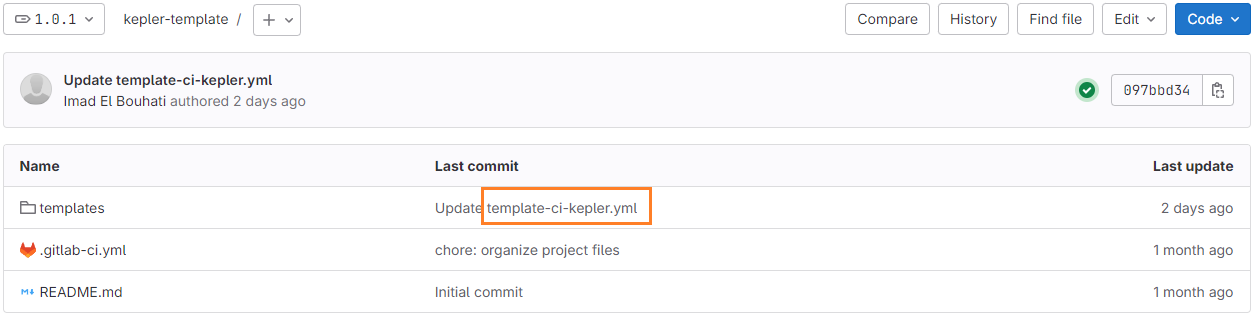
\includegraphics[width=19cm]{Figures/kepler-template-gitlab.png}
    \caption{Kepler template repository}
\end{figure}

\subsection*{Integration of the Kepler Template}

After creating the template, it can be used and integrated directly into a project. To achieve this, a few lines must be added to the \texttt{.gitlab-ci.yml} file.

First, we add the \texttt{include} directive followed by the path to our directory containing the Kepler template into an existing pipeline.

\begin{figure}[H]
  \centering
  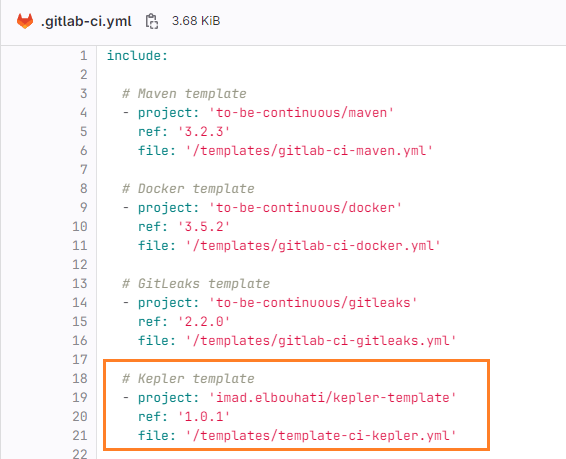
\includegraphics[width=13cm]{Figures/kepler-template-integration.png}
  \caption{Integration of the Kepler template}
\end{figure}

Next, we specify the stage name as \texttt{"deploy"}.

\begin{figure}[H]
  \centering
  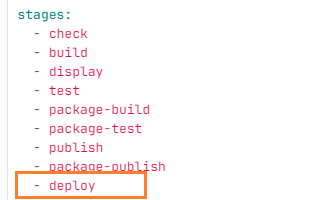
\includegraphics[width=10cm]{Figures/deploy-kepler-stage.png}
  \caption{Stage \texttt{"deploy"}}
\end{figure}

We define the following variables for the deployment:

\begin{itemize}
    \item \texttt{HELM\_RELEASE\_NAME} as the name of our Helm release.
    \item \texttt{HELM\_NAMESPACE} as the namespace for our Helm deployment.
    \item \texttt{KUBECONFIG\_CONTENT} to store cluster authentication information for kubectl.
\end{itemize}

\begin{figure}[H]
  \centering
  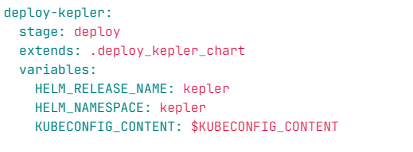
\includegraphics[width=0.8\textwidth]{Figures/deployment-variable.png}
  \caption{Deployment variables for Kepler}
\end{figure}

This configuration allows us to include the steps for deploying Kepler in our CI/CD pipeline using Helm and Kubernetes.


\section{Deploying Prometheus \& Grafana on Kubernetes}

To deploy Prometheus and Grafana in our Kubernetes cluster as part of the existing CI/CD pipeline, we have followed a structured approach. This ensures that both monitoring and visualization tools are set up correctly and efficiently.

First, we create a new job in the \texttt{.gitlab-ci.yml} file named \texttt{deploy-prometheus-grafana}. This job will run after the \texttt{deploy-kepler} job, ensuring that Kepler is deployed before Prometheus and Grafana.

\begin{figure}[H]
  \centering
  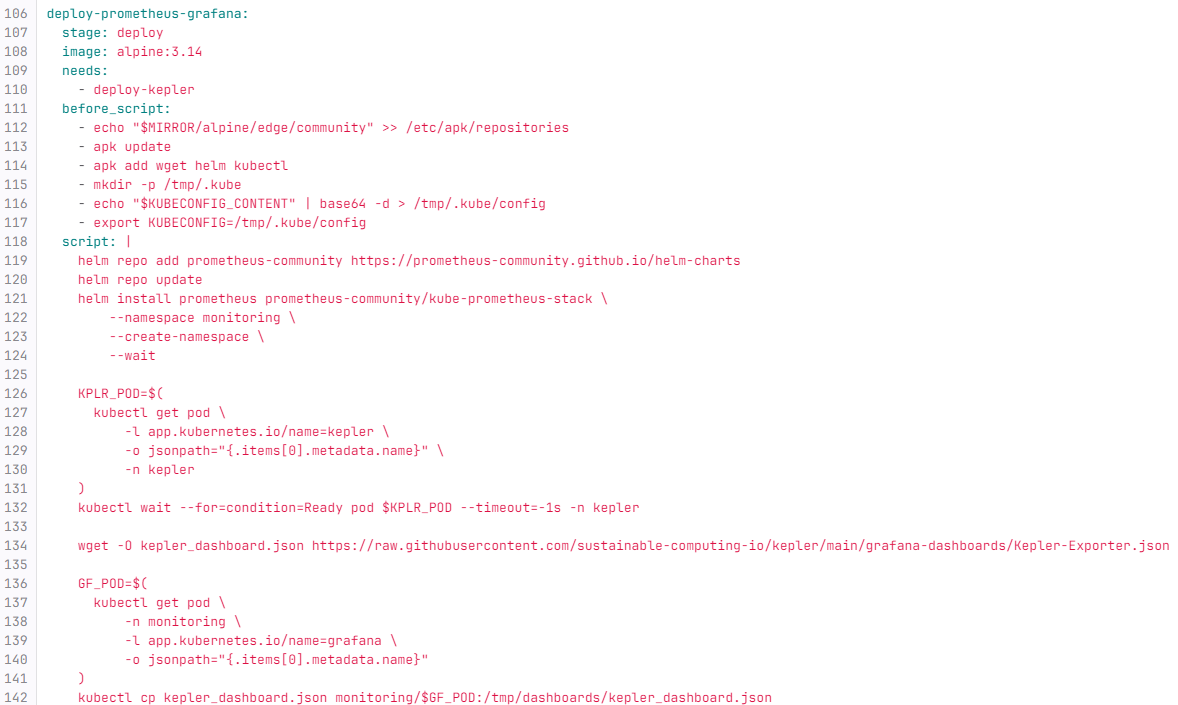
\includegraphics[width=16cm]{Figures/deploy-prometheus-grafana-job.png}
  \caption{Job \texttt{deploy-prometheus-grafana}}
\end{figure}

Next, we define the necessary configurations and scripts for deploying Prometheus and Grafana.
This script accomplishes the following:

\begin{itemize}
  \item Adds the Prometheus Helm chart repository and updates Helm repositories.
  \item Installs the Prometheus stack in the \texttt{monitoring} namespace.
  \item Waits for the Kepler pod to be ready.
  \item Downloads the Kepler Grafana dashboard JSON file.
  \item Finds the Grafana pod and copies the Kepler dashboard JSON file to it.
\end{itemize}

\section{Configuring Rules and Alerts in Prometheus}
In this section, we will cover the steps involved in configuring Prometheus to monitor specific metrics and set up alerting rules to notify us of any anomalies. Prometheus allows us to define custom rules for generating alerts based on our metrics, which can be integrated with various notification channels like Slack.

\subsection{Creating Custom Alerting Rules}

To monitor the energy consumption of our nodes, we have defined several custom alerting rules. These rules are specified in the \texttt{additionalPrometheusRulesMap} section of our Prometheus configuration. Here is an example configuration:

\begin{figure}[H]
    \centering
    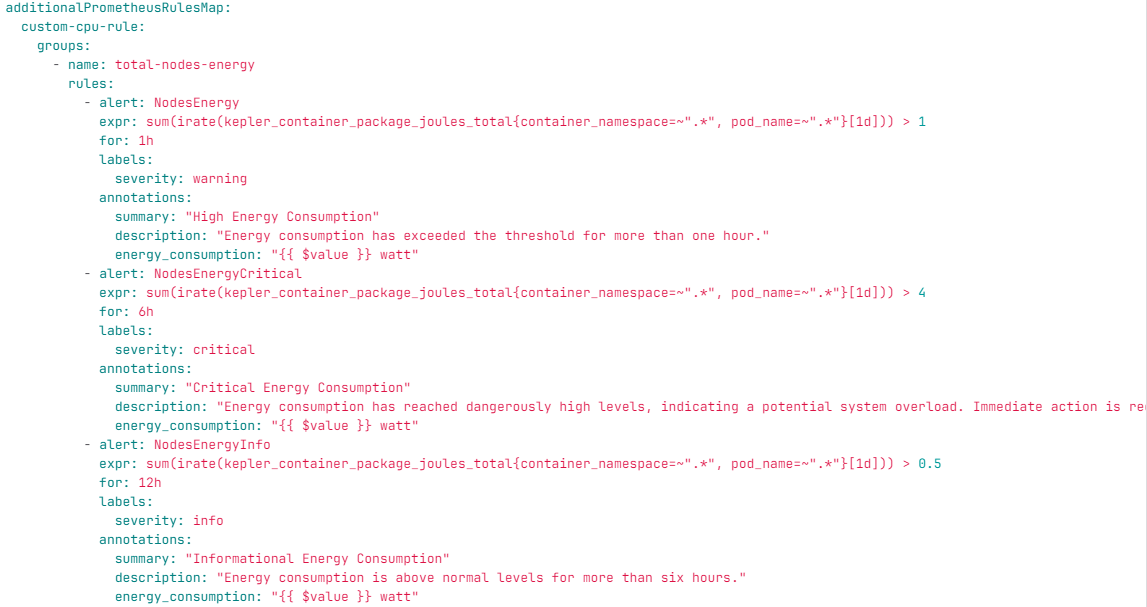
\includegraphics[width=16cm]{Figures/prometheus-rule.png}
    \caption{Prometheus rules}
\end{figure}

This configuration defines three alerts:

\begin{itemize}
  \item \textbf{NodesEnergy}: Triggered when the energy consumption exceeds 1 watt for more than 1 hour. It has a \texttt{severity} label set to \texttt{warning}.
  \item \textbf{NodesEnergyCritical}: Triggered when the energy consumption exceeds 4 watts for more than 6 hours. It has a \texttt{severity} label set to \texttt{critical}.
  \item \textbf{NodesEnergyInfo}: Triggered when the energy consumption exceeds 0.5 watts for more than 12 hours. It has a \texttt{severity} label set to \texttt{info}.
\end{itemize}

Each alert includes annotations providing a summary and description of the alert, along with the actual energy consumption value.

\begin{figure}[H]
  \centering
  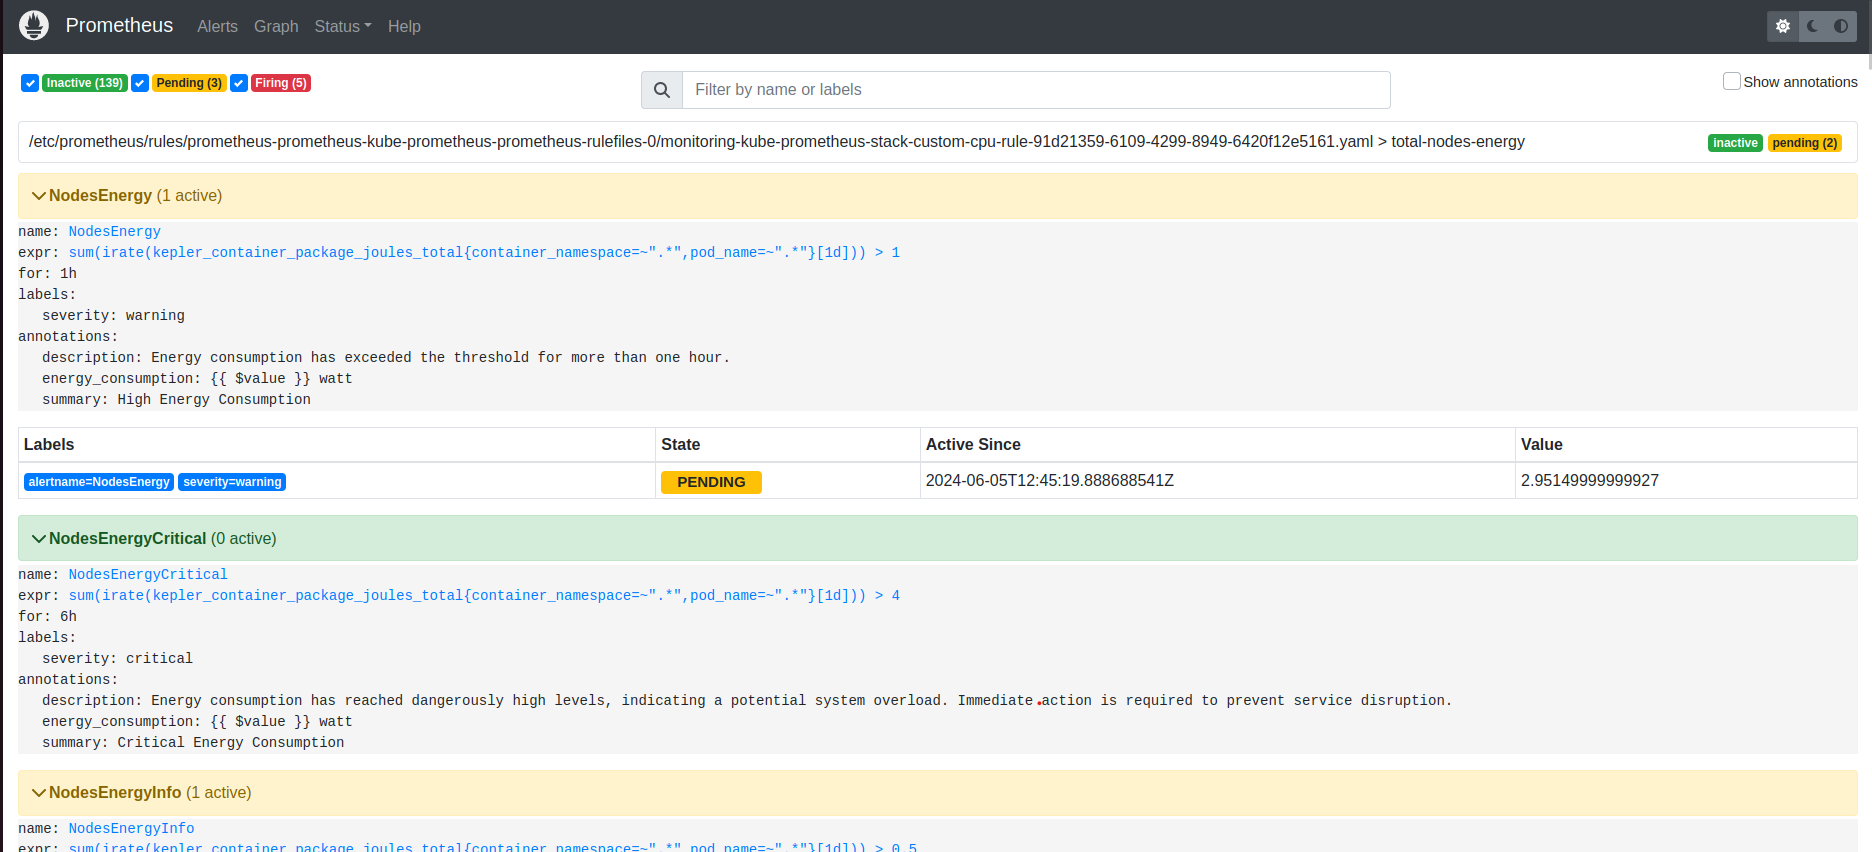
\includegraphics[width=0.8\textwidth]{Figures/alerts.png}
  \caption{Alerts dashboard in Prometheus}
\end{figure}

\subsection{Integrating Alerts with Slack}

To ensure that we receive notifications for these alerts, we integrate Prometheus with Slack using Alertmanager. The following configuration sets up Alertmanager to send alerts to a Slack channel:

\begin{figure}[H]
    \centering
    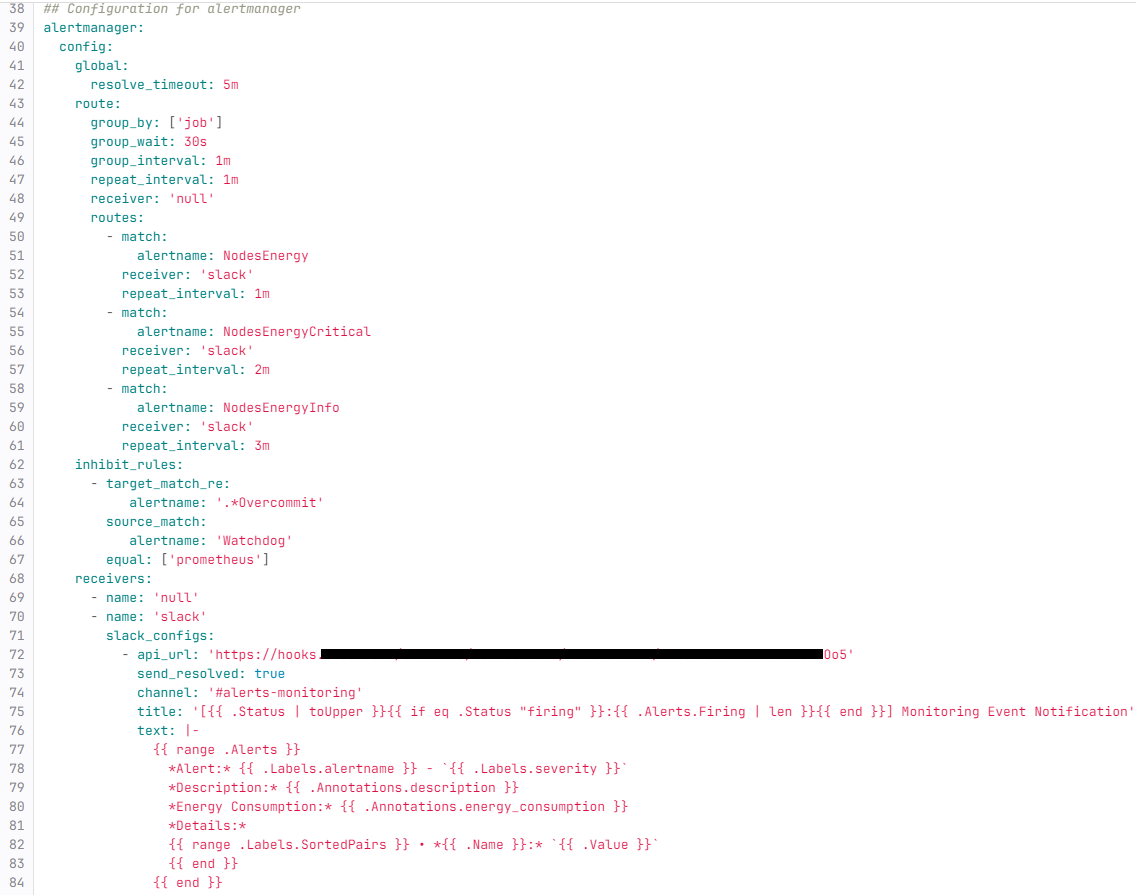
\includegraphics[width=0.8\textwidth]{Figures/alert-manager.png}
    \caption{Alert Manager Configuration}
  \end{figure}

This configuration does the following:

\begin{itemize}
  \item Sets global configuration options such as \texttt{resolve\_timeout}.
  \item Defines routing rules to determine which alerts should be sent to Slack. Alerts named \texttt{NodesEnergy}, \texttt{NodesEnergyCritical}, and \texttt{NodesEnergyInfo} are routed to the Slack receiver.
  \item Sets up inhibition rules to prevent redundant alerts.
  \item Configures the Slack receiver with a webhook URL, ensuring that alerts are sent to the \\
  \texttt{\#alerts-monitoring} channel. The \texttt{title} and \texttt{text} fields format the alert message.
\end{itemize}

\begin{figure}[H]
  \centering
  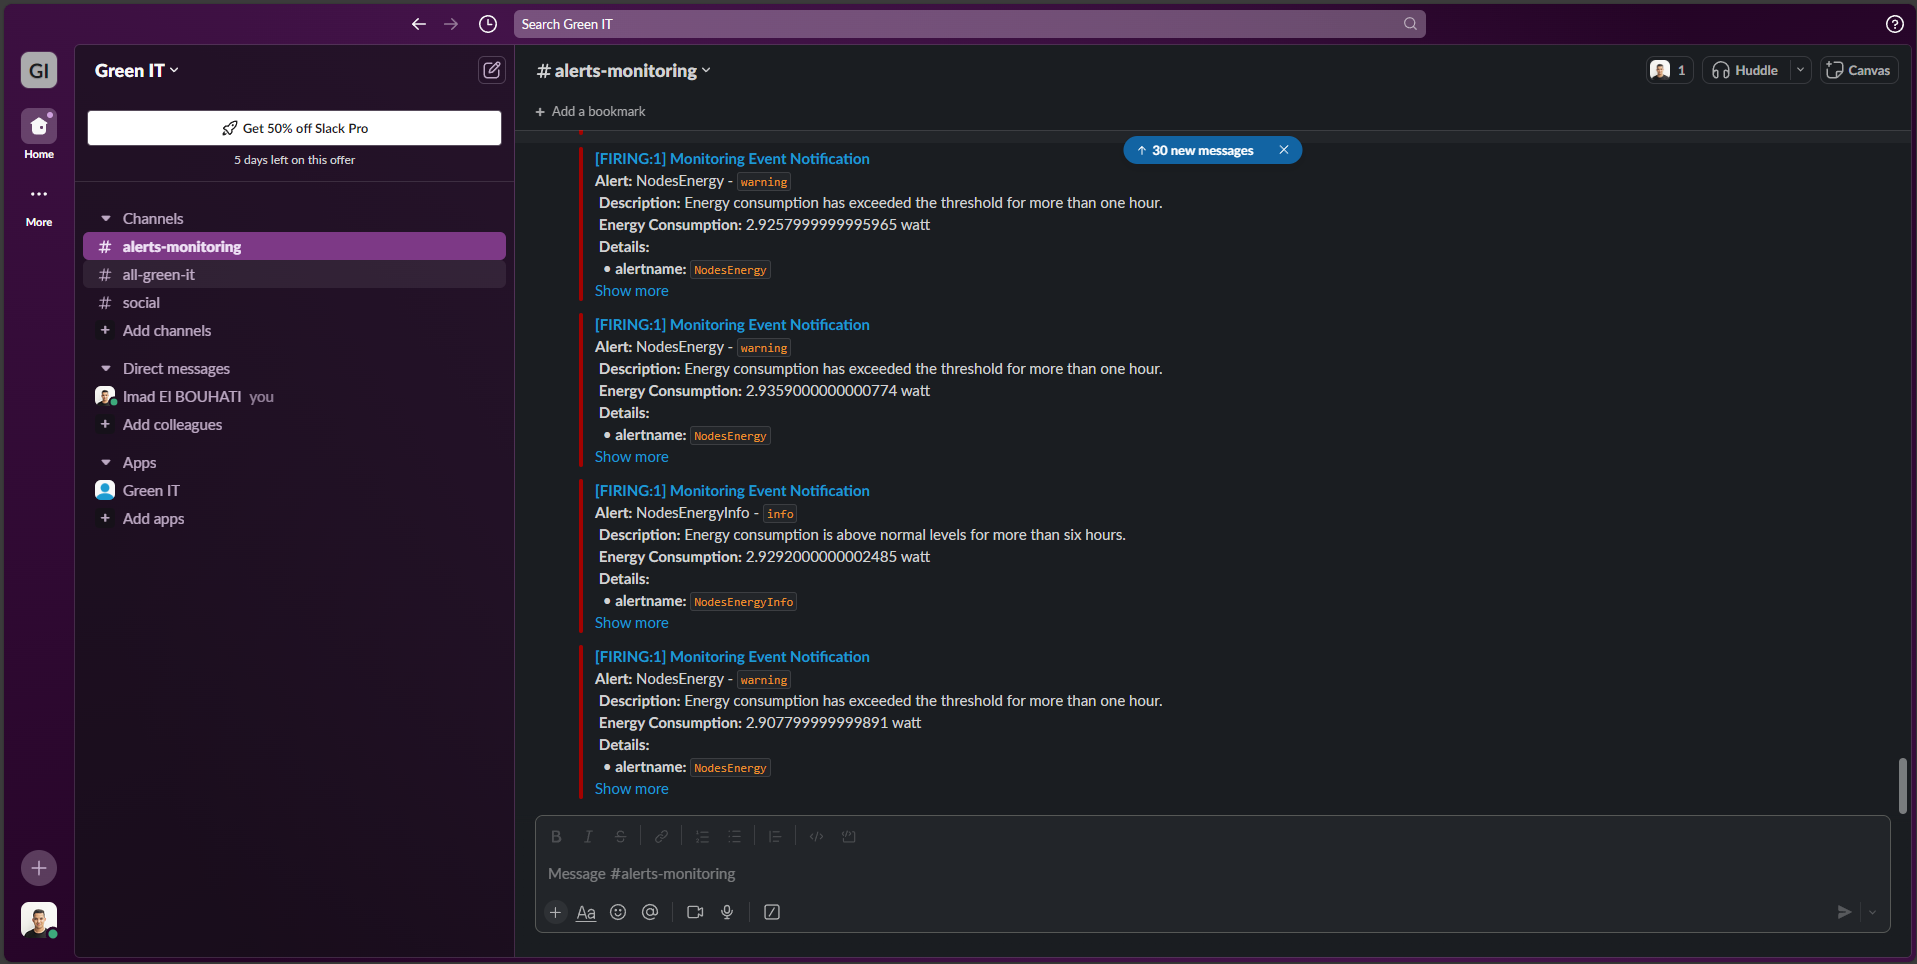
\includegraphics[width=0.8\textwidth]{Figures/slack-green-it channel.png}
  \caption{Slack alerts messages}
\end{figure}

\section{Launching the CI/CD Pipeline}

In this section, we will discuss the process of launching our CI/CD pipeline, showcasing the various stages and the resources deployed in our Kubernetes cluster. Finally, we will present the Grafana dashboard to visualize the metrics collected by Prometheus.

\subsection{Starting the GitLab Pipeline}

To start the pipeline, we push our code changes to the GitLab repository. This triggers the GitLab CI/CD pipeline, which executes the stages defined in the \texttt{.gitlab-ci.yml} file. The pipeline consists of multiple stages, including building, testing, and deploying our applications.

\begin{figure}[H]
  \centering
  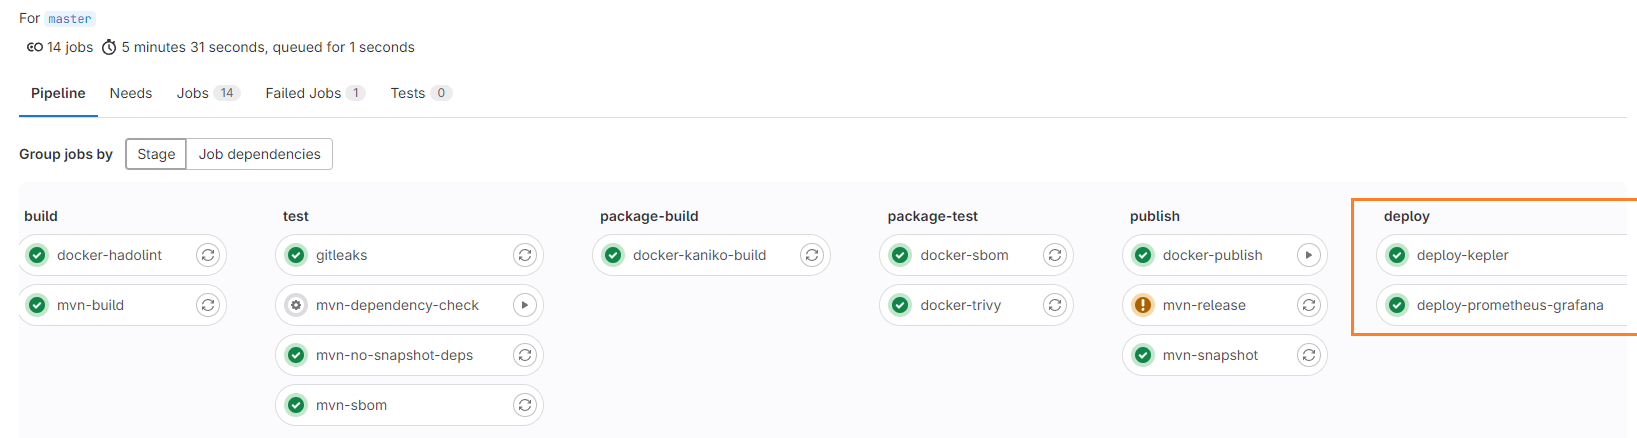
\includegraphics[width=0.8\textwidth]{Figures/gitlab-pipeline.png}
  \caption{GitLab CI/CD Pipeline Stages}
\end{figure}

\subsection{Deployed Resources in Kubernetes}

Once the pipeline completes successfully, the following resources were deployed in the `kepler` and `monitoring` namespaces within our Kubernetes cluster.

\subsubsection{Kepler Namespace}

The `kepler` namespace contains the resources related to the Kepler application. These resources include:

\begin{itemize}
    \item \textbf{Pod}: The running instance of the Kepler application.
    \item \textbf{Service}: Provides a stable IP and DNS name for accessing the Kepler application.
    \item \textbf{DaemonSet}: Ensures that a copy of the Kepler application runs on all nodes.
\end{itemize}

\begin{figure}[H]
    \centering
    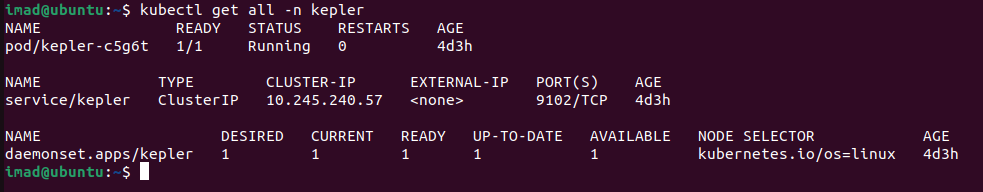
\includegraphics[width=\linewidth]{Figures/kepler-monitoring-resources.png}
    \caption{Deployed resources in the `kepler` namespace.}
    \label{fig:kepler-resources}
\end{figure}

\subsubsection{Monitoring Namespace}

The `monitoring` namespace contains the resources for monitoring and alerting. These resources include:

\begin{itemize}
    \item \textbf{Prometheus}: Collects and stores metrics data.
    \item \textbf{Alertmanager}: Manages alerts sent by Prometheus.
    \item \textbf{Grafana}: Visualizes the collected metrics.
    \item \textbf{Services}: Provide stable IPs and DNS names for accessing Prometheus, Alertmanager, and Grafana.
    \item \textbf{DaemonSet and Deployments}: Ensure that Prometheus and its components are running correctly.
\end{itemize}

\begin{figure}[H]
    \centering
    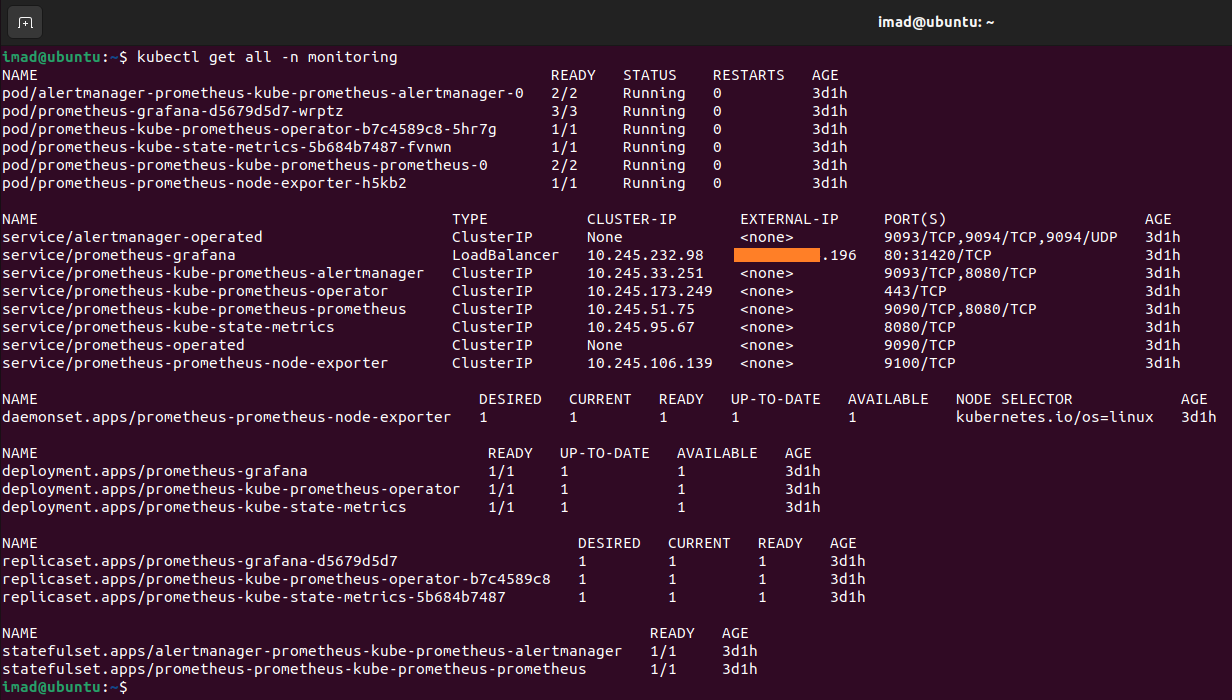
\includegraphics[width=\linewidth]{Figures/monitoring-namespace-resources.png}
    \caption{Deployed resources in the `monitoring` namespace.}
    \label{fig:monitoring-resources}
\end{figure}

\subsection{Grafana Dashboards}
We utilize Grafana dashboards to monitor the performance and resource utilization of our Kubernetes cluster. Below are the key metrics visualized:
\subsubsection{Carbon Emissions Dashboard}
\begin{figure}[H]
    \centering
    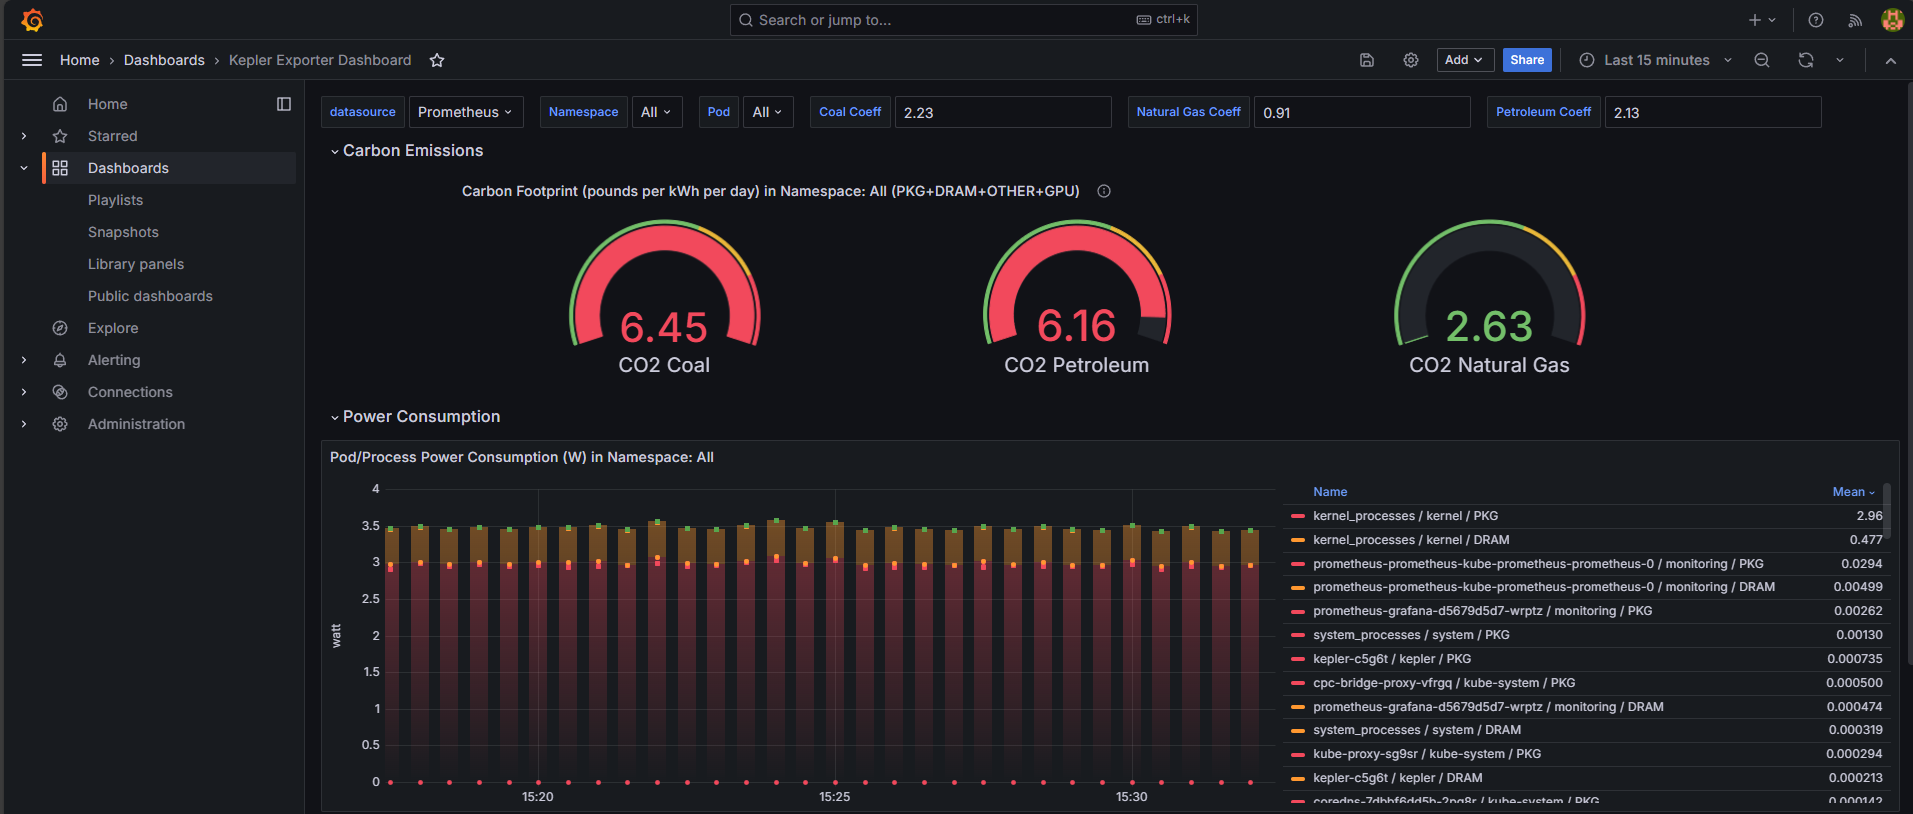
\includegraphics[width=\textwidth]{Figures/grafana-dashboard-1.png}
    \caption{Grafana dashboard showing carbon emissions based on energy consumption.}
    \label{fig:grafana-dashboard-2}
\end{figure}

The above figure (Figure \ref{fig:grafana-dashboard-2}) shows the carbon emissions associated with the energy consumption in the cluster. The dashboard highlights the carbon footprint in terms of \texttt{CO$_2$ Coal}, \texttt{CO$_2$ Petroleum}, and \texttt{CO$_2$ Natural Gas}. This information is crucial for understanding the environmental impact of our infrastructure and taking steps towards sustainability.


\subsubsection{Power Consumption Dashboard}
\begin{figure}[H]
    \centering
    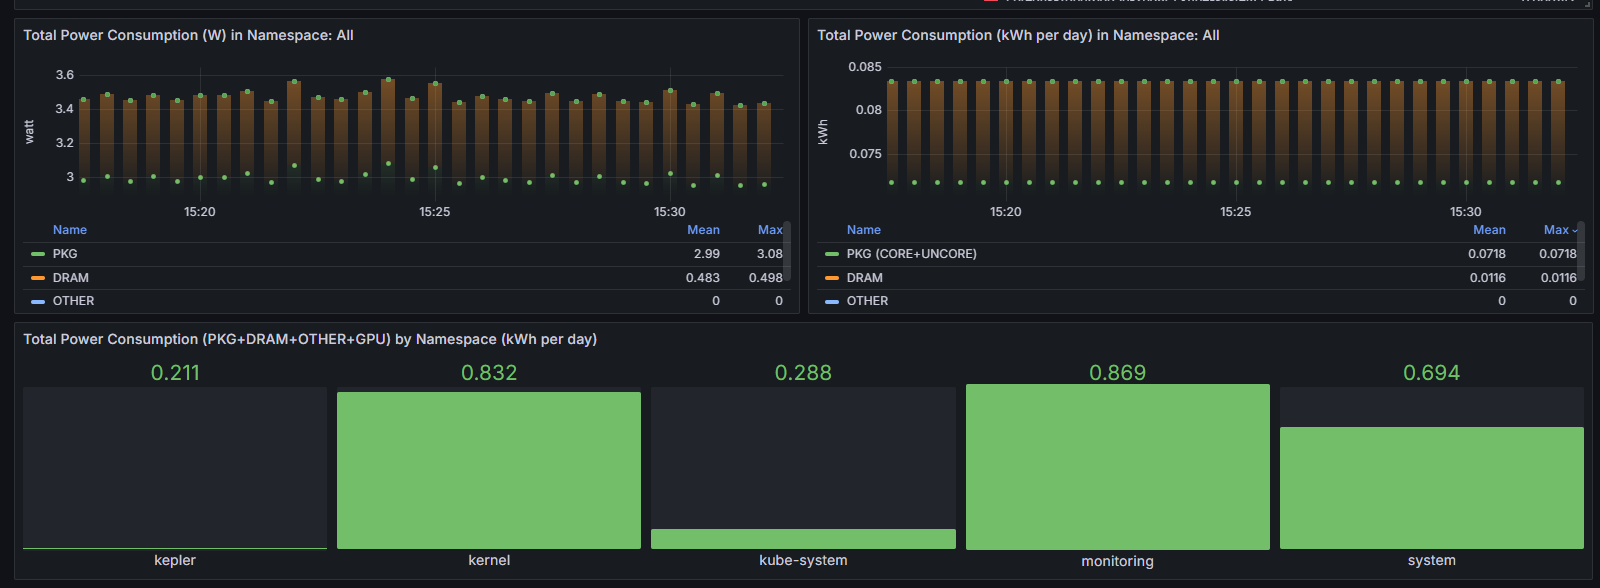
\includegraphics[width=\textwidth]{Figures/grafana-dashboard-2.png}
    \caption{Grafana dashboard showing total power consumption by namespace.}
    \label{fig:grafana-dashboard-1}
\end{figure}

The above figure (Figure \ref{fig:grafana-dashboard-1}) displays the total power consumption (in watts) across all namespaces in the cluster. The power consumption is broken down into different components: \texttt{PKG} (Package), \texttt{DRAM} (Memory), and \texttt{OTHER}. The dashboard provides insights into the energy usage trends over time, which helps in optimizing resource allocation and identifying potential inefficiencies.



\newpage

\section{Conclusion}

Integrating our CI/CD pipeline with Kubernetes and monitoring tools has enabled efficient deployment and management of large-scale resources. The \texttt{kepler} and \texttt{monitoring} namespaces hosted essential pods, services, and daemons, ensuring high availability and simplified maintenance.
The Grafana dashboards provide detailed views of power consumption and CO$_2$ emissions, facilitating proactive and sustainable infrastructure management. This approach not only optimized performance but also helped minimize the environmental impact of our operations.
Future improvements could include integrating additional monitoring features and extending our CI/CD pipeline with complementary tools to enhance the robustness and security of our Kubernetes ecosystem.

\pagebreak

\chapter*{General Conclusion and Perspectives}


% This conclusion is unnumbered, if you want it numbered, you can remove the * from above and remove the line below, so it becomes a chapter, then add sections.

\addcontentsline{toc}{chapter}{General Conclusion and Perspectives} %adds to the table of contents 

\label{chap:General Conclusion} 

Lorem ipsum dolor sit amet, consectetur adipiscing elit. Praesent nec dapibus justo. Donec sagittis vulputate ante sed porttitor. Suspendisse sit amet nisl massa. Curabitur nec nisl condimentum, egestas ex vitae, dapibus enim. Etiam iaculis, erat faucibus pellentesque sagittis, nisi justo sollicitudin nibh, et condimentum augue massa non turpis. Proin commodo enim fermentum suscipit condimentum. Maecenas molestie, dui nec vestibulum rhoncus, arcu nisl faucibus neque, a ornare nisi massa ac eros. Aenean id velit sit amet lacus mattis varius. Donec fringilla massa sed nisi eleifend, a aliquet mi tempus. Nunc posuere euismod est, nec tristique augue lobortis non. Sed sodales sem ut metus tempus ullamcorper.

Nullam fermentum id mauris suscipit varius. Quisque tristique tempor fringilla. Nam porta tincidunt orci in consectetur. Suspendisse nec sem nisi. Suspendisse potenti. Sed sodales aliquam libero, at dapibus ligula accumsan non. Quisque congue et urna a consectetur. Nullam maximus venenatis ornare. Donec in luctus urna, vel rhoncus lectus. Etiam lobortis, lacus nec gravida iaculis, magna nulla iaculis leo, quis congue nunc tortor pellentesque lorem. Sed fermentum vulputate dui, ac malesuada eros molestie sit amet. Proin fringilla elit justo, in posuere urna porttitor et. Curabitur dictum justo vitae metus pellentesque, eget feugiat sem feugiat.

Curabitur in mauris eu felis cursus auctor eget ut massa. Curabitur eleifend consectetur magna in ultrices. Etiam ut semper turpis. Morbi sed ipsum nec sem rutrum blandit sit amet vitae felis. Vestibulum vitae hendrerit diam. Aliquam pellentesque est mi, et tempus nisl laoreet in. Maecenas consequat augue a ante congue dignissim. In condimentum erat in volutpat tempus. Mauris vulputate, enim ut dignissim varius, lorem purus tristique sapien, lobortis accumsan dolor lorem quis eros. Duis vel imperdiet metus, non suscipit tortor.


%\section{Optional Section}

\appendix


%\chapter{Glossary}
\label{chap:Glossary} 


\textbf{Telnet:} Telnet is a network protocol that allows users to establish a remote terminal connection to a computer or network device over a network.\\


\textbf{SSH (Secure Shell):} SSH is a network protocol used for secure remote administration and secure file transfers.\\


\textbf{SNMP (Simple Network Management Protocol):} SNMP is a network protocol designed for managing and monitoring network devices and systems.\\


\pagebreak

\chapter{Acronyms}

\begin{tabular}{l l}

    \textbf{ACPI} & Advanced Configuration and Power Interface \\
    \textbf{AI} & Artificial Intelligence \\
    \textbf{AMOA} & Assistant à Maîtrise d'OuvrAge \\
    \textbf{API} & Application Programming Interface \\
    \textbf{AWS} & Amazon Web Services \\
    \textbf{BM} & Bare-Metal \\
    \textbf{BPF} & Berkeley Packet Filter \\
    \textbf{CD} & Continuous Delivery \\
    \textbf{CEO} & Chief Executive Officer \\
    \textbf{CI} & Continuous Integration \\
    \textbf{CNCF} & Cloud Native Computing Foundation \\
    \textbf{CO2} & Carbon Dioxide \\
    \textbf{CPU} & Central Processing Unit \\
    \textbf{DNS} & Domain Name System \\
    \textbf{DRAM} & Dynamic Random Access Memory \\
    \textbf{EC2} & Elastic Compute Cloud \\
    \textbf{EIC} & Enriched Interactions and Collaboration \\
    \textbf{GHG} & Greenhouse Gas \\
    \textbf{GPU} & Graphics Processing Unit \\
    \textbf{HTTP} & Hypertext Transfer Protocol \\

\end{tabular}

\pagebreak

\begin{tabular}{l l}
    \textbf{HR} & Human Resources \\
    \textbf{IP} & Internet Protocol \\
    \textbf{IT} & Information Technology \\
    \textbf{JSON} & JavaScript Object Notation \\
    \textbf{JVM} & Java Virtual Machine \\
    \textbf{KPI} & Key Performance Indicator \\
    \textbf{LAN} & Local Area Network \\
    \textbf{LXC} & Linux Containers \\
    \textbf{LXD} & Linux Containers Daemon \\
    \textbf{MSC} & Major Service Centers \\
    \textbf{MTTD} & Mean Time to Detect \\
    \textbf{MTTI} & Mean Time to Identify \\
    \textbf{MTTR} & Mean Time to Repair \\
    \textbf{NVML} & NVIDIA Management Library \\
    \textbf{OBS} & Orange Business Services \\
    \textbf{OCD} & Orange Cyberdefense \\
    \textbf{OCWS} & Orange Connectivity and Services Workspace \\
    \textbf{OINIS} & Orange International Networks Infrastructures and Services \\
    \textbf{PKG} & Package \\
    \textbf{RAPL} & Running Average Power Limit \\
    \textbf{REST} & Representational State Transfer \\
    \textbf{SCM} & Source Code Management \\
    \textbf{SDWAN} & Software-Defined Wide Area Network \\
    \textbf{SSH} & Secure Shell \\
    \textbf{TAAS} & Testing as a Service \\
    \textbf{TTM} & Time to Market \\
    \textbf{URL} & Uniform Resource Locator \\
    \textbf{VM} & Virtual Machine \\
    \textbf{VMM} & Virtual Machine Monitor \\
    \textbf{VPN} & Virtual Private Network \\
    \textbf{WIFI} & Wireless Fidelity \\
    \textbf{YAML} & YAML Ain't Markup Language \\
\end{tabular}

\begin{thebibliography}{99}
    \addcontentsline{toc}{chapter}{Bibliography}
    
    \bibitem{ref1}
    Julien Pivotto \& Brian Brazil, Prometheus Up \& Running.
    
    \bibitem{ref2}
    \emph{How Do You Go from DevOps to DevGreenOps?},
    \href{https://greenspector.com/en/how-do-you-go-from-devops-to-devgreenops/}{\textbf{Greenspector}}
    
    \bibitem{ref3}
    \emph{Green DevOps: Poursuivre l'excellence opérationnelle tout en réduisant l'impact environnemental},
    \href{https://glalloue.medium.com/green-devops-poursuivre-lexcellence-op%C3%A9rationnelle-tout-en-r%C3%A9duisant-l-impact-environnemental-de500cfcc9eb}{\textbf{Medium article by glalloue}}
    
    \bibitem{ref4}
    \emph{DevOps Monitoring},
    \href{https://www.splunk.com/en_us/blog/learn/devops-monitoring.html}{\textbf{Splunk Blog}}
    
    \bibitem{ref5}
    \emph{Docker Architecture Overview},
    \href{https://docs.docker.com/get-started/overview/#:~:text=with%20fewer%20resources.-,Docker%20architecture,to%20a%20remote%20Docker%20daemon.}{\textbf{Docker Documentation}}
    
    \bibitem{ref6}
    \emph{What is DevSecOps?},
    \href{https://www.redhat.com/en/topics/devops/what-is-devsecops}{\textbf{Red Hat}}
    
    \bibitem{ref7}
    \emph{Exploring Kepler's Potentials: Unveiling Cloud Application Power Consumption},
    \href{https://www.cncf.io/blog/2023/10/11/exploring-keplers-potentials-unveiling-cloud-application-power-consumption/}{\textbf{CNCF Blog}}
    
    \bibitem{ref8}
    \emph{Kepler Helm Chart Documentation},
    \href{https://github.com/sustainable-computing-io/kepler-helm-chart/blob/main/README.md}{\textbf{GitHub}}
    
    \bibitem{ref9}
    \emph{Orange Business Services},
    \href{https://www.orange-business.com/fr}{\textbf{Orange Business}}
    
    \bibitem{ref10}
    \emph{Prometheus Documentation},
    \href{https://prometheus.io/docs}{\textbf{Prometheus.io}}
    
    \bibitem{ref11}
    \emph{Slack API: Webhooks},
    \href{https://api.slack.com/messaging/webhooks}{\textbf{Slack API Documentation}}
    
    \end{thebibliography}
    

\end{document}